\documentclass[12pt]{article}
\newif\ifshowsolutions
\showsolutionsfalse
%\showsolutionstrue

%% arXiv paper template by Flip Tanedo
%% last updated: Dec 2016



%%%%%%%%%%%%%%%%%%%%%%%%%%%%%
%%%  THE USUAL PACKAGES  %%%%
%%%%%%%%%%%%%%%%%%%%%%%%%%%%%

\usepackage{amsmath}
\usepackage{amssymb}
\usepackage{amsfonts}
\usepackage{graphicx}
\usepackage{xcolor}
\usepackage{nopageno}
\usepackage{enumerate}
\usepackage{parskip}
\usepackage{comment}
	
	
%http://tex.stackexchange.com/questions/15509/hide-custom-environment-content-based-on-boolean
\ifshowsolutions
	\newenvironment{solution}%
	{\color{blue!60!black}
	\textsf{\textbf{Solution}}:
	}%
	%
	{\ignorespacesafterend}
\else
	\excludecomment{solution}
\fi
	
%\newenvironment{solution}
%    {%\begin{sol}
%    \textcolor{blue!40!black}{
%	\textbf{Solution}:}
%    }
%    { 
%    %\end{sol}
%    }
%    
%%\includecomment{solution}




%%%%%%%%%%%%%%%%%%%%%%%%%%%%%%%%%
%%%  UNUSUAL PACKAGES        %%%%
%%%  Uncomment as necessary. %%%%
%%%%%%%%%%%%%%%%%%%%%%%%%%%%%%%%%

\usepackage{titlesec}
\titleformat*{\section}{\large\bfseries}

%% MATH AND PHYSICS SYMBOLS
%% ------------------------
%\usepackage{slashed}       % \slashed{k}
%\usepackage{mathrsfs}      % Weinberg-esque letters
%\usepackage{youngtab}	    % Young Tableaux
%\usepackage{pifont}        % check marks
\usepackage{bbm}           % \mathbbm{1} incomp. w/ XeLaTeX 
%\usepackage[normalem]{ulem} % for \sout


%% CONTENT FORMAT AND DESIGN (below for general formatting)
%% --------------------------------------------------------
\usepackage{lipsum}        % block of text (formatting test)
%\usepackage{color}         % \color{...}, colored text
%\usepackage{framed}        % boxed remarks
%\usepackage{subcaption}    % subfigures; subfig depreciated
%\usepackage{paralist}      % compactitem
%\usepackage{appendix}      % subappendices
%\usepackage{cite}          % group cites (conflict: collref)
%\usepackage{tocloft}       % Table of Contents	


%% TABLES IN LaTeX
%% ---------------
%\usepackage{booktabs}      % professional tables
%\usepackage{nicefrac}      % fractions in tables,
%\usepackage{multirow}      % multirow elements in a table
%\usepackage{arydshln} 	    % dashed lines in arrays

%% Other Packages and Notes
%% ------------------------
%\usepackage[font=small]{caption} % caption font is small



%\renewcommand{\thesection}{}
%\renewcommand{\thesubsection}{\arabic{subsection}}

%%%%%%%%%%%%%%%%%%%%%%%%%%%%%%%%%%%%%%%%%%%%%%%
%%%  PAGE FORMATTING and (RE)NEW COMMANDS  %%%%
%%%%%%%%%%%%%%%%%%%%%%%%%%%%%%%%%%%%%%%%%%%%%%%

\usepackage[margin=2cm]{geometry}   % reasonable margins

\graphicspath{{figures/}}	        % set directory for figures

% for capitalized things
\newcommand{\acro}[1]{\textsc{\MakeLowercase{#1}}}    

\numberwithin{equation}{section}    % set equation numbering
\renewcommand{\tilde}{\widetilde}   % tilde over characters
\renewcommand{\vec}[1]{\mathbf{#1}} % vectors are boldface

\newcommand{\dbar}{d\mkern-6mu\mathchar'26}    % for d/2pi
\newcommand{\ket}[1]{\left|#1\right\rangle}    % <#1|
\newcommand{\bra}[1]{\left\langle#1\right|}    % |#1>
\newcommand{\Xmark}{\text{\sffamily X}}        % cross out

% Change list spacing (instead of package paralist)
% from: http://en.wikibooks.org/wiki/LaTeX/List_Structures#Line_spacing
%\let\oldenumerate\enumerate
%\renewcommand{\enumerate}{
%  \oldenumerate
%  \setlength{\itemsep}{1pt}
%  \setlength{\parskip}{0pt}
%  \setlength{\parsep}{0pt}
%}

\let\olditemize\itemize
\renewcommand{\itemize}{
  \olditemize
  \setlength{\itemsep}{1pt}
  \setlength{\parskip}{0pt}
  \setlength{\parsep}{0pt}
}


% Commands for temporary comments
\newcommand{\flip}[1]{{\color{red} [\textbf{Flip}: {#1}]}}
\newcommand{\email}[1]{\texttt{\href{mailto:#1}{#1}}}

\newenvironment{institutions}[1][2em]{\begin{list}{}{\setlength\leftmargin{#1}\setlength\rightmargin{#1}}\item[]}{\end{list}}


\usepackage{fancyhdr}		% to put preprint number



% Commands for listings package
%\usepackage{listings}      % \begin{lstlisting}, for code
%
% \lstset{basicstyle=\ttfamily\footnotesize,breaklines=true}
%    sets style to small true-type


%%%%%%%%%%%%%%%%%%%%%%%%%%%%%%%%%%%%%%%%%%%%%%
%%%  TIKZ COMMANDS FOR EXTERNAL DIAGRAMS  %%%%
%%%  requires -shell-escape               %%%%
%%%  in texpad 1.7: prefs > shell esc sec %%%%
%%%%%%%%%%%%%%%%%%%%%%%%%%%%%%%%%%%%%%%%%%%%%%

%% This is for exporting tikz figures as into a ./tikz/ subfolder.
%% It is useful if you want pdf versions of the tikz diagrams or
%% if you need to speed up compilation of a large document with
%% many tikz diagrams.

%\write18{} % Careful with this!
%\usetikzlibrary{external}
%\tikzexternalize[prefix=tikz/] % folder for external pdfs


%%%%%%%%%%%%%%%%%%%
%%%  HYPERREF  %%%%
%%%%%%%%%%%%%%%%%%%

%% This package has to be at the end; can lead to conflicts
\usepackage{microtype}
\usepackage[
	colorlinks=true,
	citecolor=black,
	linkcolor=black,
	urlcolor=green!50!black,
	hypertexnames=false]{hyperref}



%%%%%%%%%%%%%%%%%%%%%
%%%  TITLE DATA  %%%%
%%%%%%%%%%%%%%%%%%%%%

%%% PREPRINT NUMBER USING fancyhdr
%%% Don't forget to set \thispagestyle{firststyle}
%%% ----------------------------------------------
%\renewcommand{\headrulewidth}{0pt} % no separator
%\fancypagestyle{firststyle}{
%\rhead{\footnotesize \texttt{UCI-TR-2016-XX}}}

\renewcommand{\thesubsection}{\thesection.\alph{subsection}}

\begin{document}

%\thispagestyle{empty}
%\thispagestyle{firststyle} %% to include preprint

\begin{center}

    {\Large \textsc{Homework 5:} 
    \textbf{Killing Fields, Black Holes}}


    
\end{center}

\vskip .4cm

\noindent
\begin{tabular*}{\textwidth}{rlcrll}
	\textsc{Course:}& Physics 208, {General Relativity} (Winter 2017)
	&
%	\hspace{1.2cm}
	&
	\\
	\textsc{Instructor:}& Flip Tanedo (\email{flip.tanedo@ucr.edu})
	&
	%\hfill
	&
	& 
	\\
	\textsc{Due Date:}& Tuesday, Feb 21 in class... or, you know, like... whenever.
	&
	%\hfill
	&
	%	
\end{tabular*}

You are required to complete the {\textsf{Reading Assignment}} and {\textsf{Essential Problems}} below. 
%
Please let me know if these are too time intensive. %\footnote{The `essential problems' are meant to be a bare minimum of independent work to follow the course.}.
%
You are invited to explore the `extra' problems as they apply to your goals for this course: {\textsf{Mathematical Problems}} develop geometric intuition, while {\textsf{Phenomenological Problems}} are applications of relativity. 
% 



\vspace{2em}
{\Large\textbf{\textsf{Reading Assignment}}}

Read the following topics. You may choose to read the analogous topics in an appropriate textbook or reference of your preference. Most of this reading is meant to be complementary to the approach in the lectures.

\begin{itemize}
	\item Finish chapter 12 of Hartle
	\item We will not spend much time on more realistic black holes, but feel free to peruse chapters 13 -- 15 as you are interested. For an excellent set of lecture notes, see \texttt{gr-qc/9707012}.
	\item You can start reading chapter 18 on cosmological models---we will not discuss them too much in class, but we will play with FRW metrics in upcoming homework. 
	\item The Einstein equation, which we are rapidly approaching, is described in chapter 21.
\end{itemize}

\vspace{2em}

The Schwarzchild metric is:
\begin{align}
	ds^2 = \left(1-\frac{r_s}{r}\right)dt^2 
	- \left(1-\frac{r_s}{r}\right)^{-1}dr^2
	- r^2 d\Omega^2 \ .
\end{align}
We've written $r_s = 2GM$ as the Schwarzschild radius.


\textsc{Caveat emptor}: as always, do what I mean, not necessarily what I say.


\vspace{2em}
{\Large\textbf{\textsf{Essential Problems}}}

\section{Schwarzschild Coordinate Time as $r\to r_s$}

% D'Inverno 16.5

Consider a test particle dropped at radius $r_0$ away from a Schwarzschild black hole. The particle has a conserved energy that is chosen so that it has zero initial velocity at infinity. We showed in class that the velocity in the test particle's frame is
\begin{align}
	\frac{dr}{d\tau} = \sqrt{\frac{r_s}{r}} \ .
\end{align}
This is perfectly well behaved as $r$ passes through the Schwarzschild radius, $r_s$. In this problem, we check what an observer\footnote{The observer is stationary in the Schwarzschild coordinates. For example, it is at some finite $r_\text{obs}$ and in an accelerated frame or otherwise sufficiently far away from the black hole that the acceleration from the black hole is negligible.} Use the energy conservation condition to show that
\begin{align}
	\frac{dt}{dr} = \frac{dt/d\tau}{dr/d\tau} = 
	-  \frac{\sqrt{r/r_s}}{1-r_s/r} \ .
\end{align}
Integrate this to obtain:
\begin{align}
	t-t_0 = -\frac{2}{3\sqrt{r_s}} \left(
		r^{3/2} - r_0^{3/2} + 3r_s\sqrt{r} - r_s\sqrt{r_0}
	\right)
	+ 2m \ln \frac{
	\left(\sqrt{r}+\sqrt{r_s}\right)
	\left(\sqrt{r_0}-\sqrt{r_s}\right)
	}{
	\left(\sqrt{r_0}+\sqrt{r_s}\right)
	\left(\sqrt{r}-\sqrt{r_s}\right)
	} \ .
\end{align}
Okay, you don't actually have to integrate that by hand. Use \emph{Mathematica}. Or just check the result by integrating. Don't squander your youth. However, \emph{do} plot $t(r)$ and $\tau(r)$ on the same plane to explicitly show that one is perfectly well behaved and the other gets cranky as $r\to r_s$. 

Recall that the solution for $\tau(r)$ was
\begin{align}
	\tau - \tau_0 = \frac{2}{3\sqrt{s}} \left(r_0^{3/2} - r^{3/2}\right) \ .
\end{align}

\section{Finishing your thesis when you're doomed}

You accidentally fall into the event horizon of a black hole. Perhaps experimental observations of black hole event horizons are part of your dissertation. You want to finish writing your thesis before you reach the singularity. You have reasonable booster rockets on your spaceship. What is your best strategy to make sure you \emph{maximize your time} to finish writing your thesis\footnote{Sure, nobody outside the event horizon will be able to read it and eventually you'll die... but this is how most people feel about their thesis, even in Minkowski space.}?

\section{All of those coordinate transformations}

In class we went through a series of coordinate transformations to understand the nature of the event horizon of a Schwarzschild black hole. Please go through the exercise of re-deriving the following quantities. Note: you can leave $r$ as an implicit function of each coordinate system so that, for example, you can just write $-r^2d\Omega^2$.
\begin{enumerate}
	\item In \textbf{tortoise coordinates}, we introduced 
	\begin{align}
		\tilde r = r + 2r_s \log\left(\frac{r}{r_s}-1\right)\ ,
	\end{align}
	where `log' means natural log. Derive the metric in $(t,\tilde r)$ coordinates and argue that this form means that light cones do not get `smushed' as $r\to r_s$. 
	\item Write the metric in \textbf{Eddington--Finkelstein} coordinates, $(u,r)$, where 
	\begin{align}
		v = t + \tilde r \ .
	\end{align}
	What are the slopes of the lightcones, $dv/dr$ in these coordinates? Thus argue that these coordinates describe a spacetime where things from $r>r_s$ can fall into $r<r_s$. 
	\item As we tried to derive a maximally extended description of Schwarzschild spacetime, we proposed using $u$ and $v$ coordinates:
	\begin{align}
		v &= t + \tilde r   & u & = t- \tilde r \ .
	\end{align}
	The coordinate $r$ is implicitly defined from $(v-u)$; argue that $r=r_s$ is pushed to infinity in these coordinates. Note that the `infinity' is a logarithmic divergence. Write the metric in these coordinates.
	\item To pull the event horizon back from infinity, we proposed exponentiated coordinates:
	\begin{align}
	\tilde v &= e^{v/2r_s}	
	& \tilde u = - e^{-u/2r_s} \ .
	\end{align}
	Write $\tilde v$ and $\tilde u$ in terms of the original $(r,t)$ coordinates. Write the metric in $(\tilde u, \tilde t)$ coordinates.
	\item Finally, we moved to \textbf{Kruskal} coordinates which had a timelike and spacelike direction (rather than two null or `lightcone' directions),
	\begin{align}
		T &= \frac{\tilde v + \tilde u}{2}
		&
		R &= \frac{\tilde v - \tilde u}{2} \ .
	\end{align}
	Write these in terms of the original $(r,t)$ coordinates. Write the metric in $(R,T)$ coordinates. 
	\item Draw the maximally extended Schwarzschild spacetime as given by Kruskal coordinates. Draw the event horizon.   Draw lines of constant $t$. Draw lines of constant $r$, including the singularity $r=0$. Identify the four regions as `inside the black hole', `inside a white hole', and two causally disconnected spacetime regions. 
\end{enumerate}

%\section{The Fate of the Universe}
%
%Carroll Ch. 8-1


%\section{de Sitter space}
%
%%Carroll Ch. 8-1
%de Sitter space is a maximally symmetric spacetime that can be understood as an embedding of a 4D spacetime into a flat 5D spacetime. Consider flat 5D Minkowski space,
%\begin{align}
%	ds^2 = du^2 - dx^2 - dy^2 -dz^2 = dw^2 \ .
%\end{align}
%Define a hyperboloid by
%\begin{align}
%	-u^2 + x^2 + y^2 + z^2 + w^2 = -\alpha^2 \ .
%\end{align}


\vspace{2em}
{\Large\textbf{\textsf{Phenomenological Problems}}}

\section{Killing vectors of 3D}

\textsc{Hartle Example 8.6 \& Problem 8.8.} We motivated Killing vectors as directions that leave the metric unchanged (isometries). We argued that in $D$ dimensions, there are at most $\frac 12 d(d+1)$ Killing vectors. Consider 3D flat space, $ds^2 = dx^2 + dy^2 + dz^2$. The three `obvious' Killing vectors are in the three Cartesian directions since the metric is independent of these coordinates. Shift to spherical coordinates: identify another Killing vector. Based on this, what are the two remaining Killing vectors? (You may answer either explicitly or qualitatively.)



%From the point of view of a variational principle to find geodesics, we had a `Lagrangian' $L(x,\dot x) = g_{\mu\nu}\dot x^\mu \dot x^\nu$, where $\cdot = d/d\tau$ (proper time derivative). The Euler--Lagrange equations told us that conserved quantities

\section{Gravitational Redshift}

Consider the gravitational redshift of a photon in a Schwarzschild spacetime (\textsc{Hartle section 9.2}). The time direction is a good Killing vector, $K_{(t)}$ so that $K_{(t)}\cdot p$ is a conserved quantity. 

An observer with 4-velocity $u$ observes the photon with energy $E= p\cdot u$. This is what the observer identifies with $\hbar \omega$. Recall that $u^2 = 1$ (why?). Using the Schwarzschild metric, show that
\begin{align}
u^\mu = \left(1-\frac{rs}{r}\right)^{-1/2} K_{(t)}^\mu\ .
\end{align}

What is the ratio of photon frequencies $\omega$ measured by an observer at some position $r=R$ versus $r=\infty$ (where $\infty$  means `very far away where space is effectively Minkowski')?

Compare this to what we calculated in class using the principle of equivalence in the background of a Newtonian source:
\begin{align}
	\omega_\infty = \left(1-\frac{GM}{R}\right)\omega_R \ .
\end{align}

%\section{Gravitational Collapse}



\vspace{2em}
{\Large\textbf{\textsf{Mathematical Problems}}}


\section{Killing Vectors of Spherical Symmetry}

% Carroll p 138, 198
Consider the Killing vectors in Problem 4. Show that the three rotations may be written in spherical coordinates as
\begin{align}
R &= \partial_\phi
&
S &= \cos\phi \; \partial_\theta - \cot \theta \sin \phi\; \partial_\phi
&
T &= -\sin\phi \; \partial_\theta - \cot\theta\cos\phi \; \partial_\phi \ .	
\end{align}
Calculate the commutators (Lie derivatives) of these fields. Do these look familiar from quantum mechanics? This is the algebra\footnote{\textbf{Lie groups} are groups that are also manifolds. The \textbf{Lie algebra} of the group is precisely the set of Lie derivatives at the origin. Often representation theory of continuous groups is associated more closely with discrete group theory, but in many ways it is naturally understood as a funny manifold.} of SU(2).



\section{Building a Maximally Symmetric Space}

% http://physics.stackexchange.com/questions/99882/how-to-prove-that-a-spacetime-is-maximally-symmetric

One trick to construct a maximally symmetric $d$-dimensional space is to embed it into a flat $(d+1)$-dimensional space. Consider, once again, flat 3D space. This is maximally symmetric, you identified the $\frac 12 d(d+1)$ Killing vectors in problems 4 and 6.  From this we can construct a maximally symmetric, curved 2D space by imposing a constraint
\begin{align}
	x^2 + y^2 + z^2 = R^2 \ .
\end{align}
By imposing this constraint we have broken many of isometries of the 3D space. Which isometries are broken? (Which Killing vectors are not Killing vectors of the constrained 2D space?) How many Killing vectors are left over? Based on the number of Killing vectors and the dimensionality of the space, argue that the sphere is maximally symmetric.

\textsc{Remark}: de Sitter and anti-de Sitter space are maximally symmetric 4D spacetimes that are formed analogously by considering 5D Minkowski space and projecting onto hyperboloid-y submanifolds. 



\section{Lie Derivatives and the Parallel Parking Problem}

\textsc{This question was originally on the Physics 231 homework set (Fall 2016, HW7).}

Southern California was the birthplace of car culture in the United States\footnote{Uh... citation needed. What do I look like, a historian?}. One of the consequences is that Southern Californians are notoriously bad at parallel parking---\emph{fit my car in there? That's impossible!} The point of this problem is to mathematically prove that parallel parking into a space that is strictly greater than the length of your car is possible.

This problem is essentially exercise 11.1 in Stone and Goldbart, the discussion in the book may be useful. Recall from lecture that parking a car is an \emph{anholonomic} system. The configuration space of a car is four-dimensional, given by the position of the car (say the center of mass, or the center of the rear axle), the angle with respect to some reference axis (say, the sidewalk), and the angle of the front wheels used for steering. Call these $(x,y,\theta,\phi)$, as shown in the figure.

\begin{figure*}
\begin{center}
	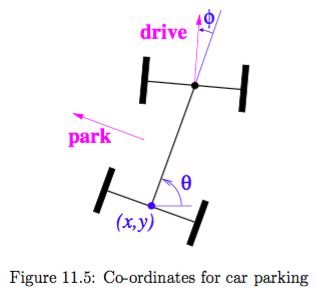
\includegraphics[width=.5\textwidth]{StoGo11}
	\caption{Fig.~11.5 from Stone \& Goldbart. Coordinates for car parking.}
	\end{center}
\end{figure*}

A convenient basis of vector fields are:
\begin{align}
	\text{\textbf{drive}} &= \cos \phi \left(\cos \theta \frac{\partial}{\partial x} + \sin \theta \frac{\partial}{\partial y}\right) + \sin \phi \frac{\partial}{\partial \theta}
	\\
	\text{\textbf{steer}} &= 
	\frac{\partial}{\partial \phi}
	\\
	\text{\textbf{skid}} &= 
	-\sin\phi \left(\cos \theta \frac{\partial}{\partial x} + \sin \theta \frac{\partial}{\partial y}\right)
	+ \cos\phi \frac{\partial}{\partial_\theta}
	\\
	\text{\textbf{park}} &= -\sin \theta \frac{\partial}{\partial x} + \cos \theta \frac{\partial}{\partial y} \ .
\end{align}
Calculate the Lie brackets of all combinations of these vector fields. There are six to calculate.

A driver can only use $\pm$\textbf{drive} and $\pm$\textbf{steer} to maneuver the car. Use the geometric interpretation of the Lie bracket (commutator) to explain how a suitable sequence of motions (forward, reverse, and turning the steering wheel) can be used to move the car \emph{sideways} into a parking space. 

Advice from Burke, \emph{Applied Differential Geometry} (1985, p. 133):
\begin{quote}
	Just remember to steer, drive, steer back, drive some more, steer, drive back, steer back, drive back: $SDS^{-1}DSD^{-1}S^{-1}D^{-1}$. You have to reverse steer in the middle of the parking place. This is not intuitive, and no doubt is part of the problem with parallel parking. Thus from only two controls you can form the vector fields \textbf{steer}, \textbf{drive}, \textbf{rotate}, and \textbf{slide}\footnote{Burke uses a slightly different set of vector fields than Stone \& Goldbart.}, which span the full tangent space at every point. You can move anywhere in the four-dimensional configuration space.
\end{quote}

If you need more help, you can try looking for discussions on the web. Here are a couple:
\begin{itemize}
	\item \url{https://www.math.wisc.edu/~robbin/parking_a_car.pdf}
	\item \url{https://rigtriv.wordpress.com/2007/10/01/parallel-parking/} .
\end{itemize}


%extra credit: parallel parking

%http://physics.stackexchange.com/questions/99882/how-to-prove-that-a-spacetime-is-maximally-symmetric



%
\end{document}